%TEX root = ../dissertation.tex

\chapter{Solution}
\label{chapter:proposed_solution}

Before attempting to develop a protocol, or solution, that meets our goals and properly addresses the problems and attacks described in the previous chapters, it is important to define the scope of our work.\\ A common appropriate way to do so is by presenting both a scenario and architecture of the solution. The Internet of Things is currently a hot trend and this work could potentially apply and benefit a wide spectrum of applications, ranging from home environments to large enterprise networks. However, these are domains that have different requirements. A home application should be easy to setup and not require complex configurations to the user. An enterprise solution can benefit from additional administrative configurations as long as the deployment of the devices can be done quickly and easily due to their potential large number. Our work will position itself in the middle of these two domains. We are looking at a complexity and number of devices greater than a home environment but it is not our focus to provide solutions for enterprise networks and their deployment restrictions. It is our belief that a Smart University Campus is an adequate scenario because it is a known environment, open to innovation and with multiple buildings, each with its connection needs. These characteristics make it a privileged scenario to effectively demonstrate the needs targeted by our work. In the following sections we will apply the information gathered in the related work sections to formally define what we are trying to achieve, what are the difficulties in achieving those goals and how can we overcome them. Then, a model of a campus with the proposed energy-efficient network architecture will be presented and their component roles explained. 

\section{Objectives and Requirements}
\paragraph{}
One of the major concerns regarding \gls{IoT} application is the communication model. For our work, we pose as requirement that the system is power-aware and uses the minimum energy possible. Additionally, the following set of objectives is desirable to build trust and allow secure communications to take place.

\begin{itemize}
	\item Confidentiality: Without confidential message transmission, packets would flow in the network in plain text. Attackers could sniff the packets in order to obtain information, and depending on the application, this could be a security breach. Even if there is no critical data being sent, privacy is still compromised.\\
	\item Integrity: Assuring message integrity means that the message was not modified between the source and its destination. Without integrity we could not rely on the received data since it could have been, intentionally or not, modified on the fly, and be providing the system wrong information.\\
	\item Authentication: The studied type of networks relies on hop-to-hop communication, meaning several nodes will take place in forwarding a packet. If they are not authenticated they could perform a wide range of attacks and disrupt the network.
\end{itemize}

\section{System Architecture and Message Flow}
\paragraph{}

As stated in the beginning of the chapter, we will use a Smart Campus scenario. Being aware of the technological improvements on sensor networks and building management technologies, the \gls{IST} administration decided to improve the monitoring of the overall conditions of the buildings and inside environments in order to better preserve its assets. To cope with the new requirements, we propose a solution for the monitoring of the campus sections by deploying a wireless sensor network on each building, connected to a central management station operated by the available staff. The scenario will be based on the \gls{IST} campus model. An overview of the system and its components over the \gls{IST} blueprints can be found in Figure \ref{fig:global_architecture}. Regarding each individual component:

\begin{itemize}
	\item Numeric Nodes: Represent the network sensor nodes, the most constrained element of the network. They cooperate to build the topology and route messages hop-by-hop until the root is reached. These are fully equipped with the energy efficient protocol stack defined in Section 4.1;\\
	\item Alphabetical Nodes: Represent the root node of each section network topology. They are equipped with the same stack of the numbered nodes but are more powerful, preferentially not battery powered and act as the bridge between the constrained 6LoWPAN environment and the central management station. These nodes must be more powerful than the numeric ones so that they can process all the requests between a group of sensors and the management station. Also, although the numeric nodes use low-power wireless radios, the alphabetical nodes must be capable of interfacing with more power hungry radios and protocols therefore requiring more resources. This differentiation allows numeric nodes (the large portion of the network devices) to keep their very constrained nature, consuming less energy, an still be able to communicate with external devices.\\
	\item Management Station: A black box model of the core components of the system. Each building reports to the central station and the staff monitors the status through it. A white box model will be shown in the following sections.\\
	\item Client: The system's clients can be any user with access credentials, but mostly the staff members. They can access the management station either from within the local network or from outside through the Internet.
\end{itemize}

\vspace{25mm} %5mm vertical space 
 
\begin{figure}[h]
  \centering
  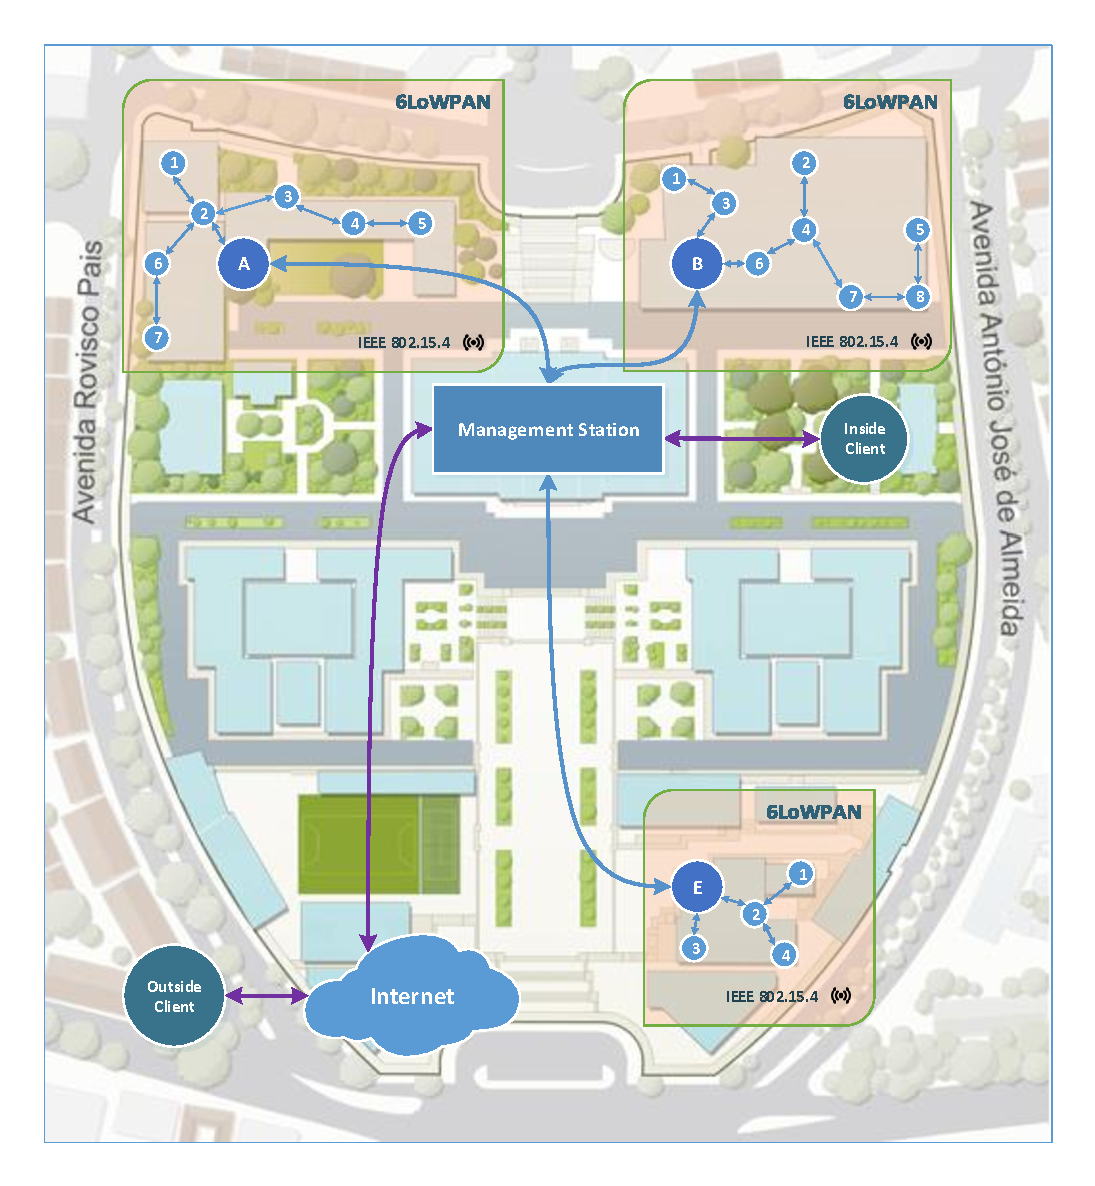
\includegraphics[width=0.9\linewidth]{figures/Global_Architecture.pdf}
  \caption{Global System Architecture}
  \label{fig:global_architecture}
\end{figure}

\paragraph{\textbf{Central Management Station}}
\paragraph{}

The central management station is divided in five main components. A white box schematic of the core components and interactions can be found in Figure \ref{fig:core_components}. Regarding each individual component:

\begin{itemize}
	\item Key Store: This component is responsible for storing the shared network key for the RPL protocol and a mapping between each network device and its key pair. This information is provided to the Client Observer for creating a secure connection to each sensor node;\\
	\item Bootstrapper: The bootstrapper acts as the interface between the management station and the network devices. It generates the device key pair and writes it together with the shared network key and the Client Observer public key into the new device;\\
	\item CoAP Client Observer:  The one and only client in the network. Instead of the user directly requesting the sensor readings, the client will observe each resource and be notified of the new value. Each time it receives an update, it stores the information on the Data Server for the clients to use;\\
	\item Data Server: A database with mappings of each node to the most up to date value reported. It's updated by the client observer and fetched on demand by the users;\\
	\item Proxy: Responsible for bridging requests coming from the Internet to the Data Server. Responsible for authenticating the external clients and providing access to the Data Server information.\\
\end{itemize}

Although each user could access the system through a \gls{CoAP} terminal and request the most up-to-date readings from the sensor nodes, this approach would cause many overheads in the system. Firstly, and since many clients can connect from different locations, many requests would be performed to the sensor nodes for the same information. Additionally each sensor node would need to be pre-installed with the public keys of all the different user terminals. This would mean additional memory usage in the physical devices, and more requests to the already constrained battery operated network. With the single client approach acting as an observer, only one message needs to go through the network for each new reading.

\begin{figure}[h]
  \centering
  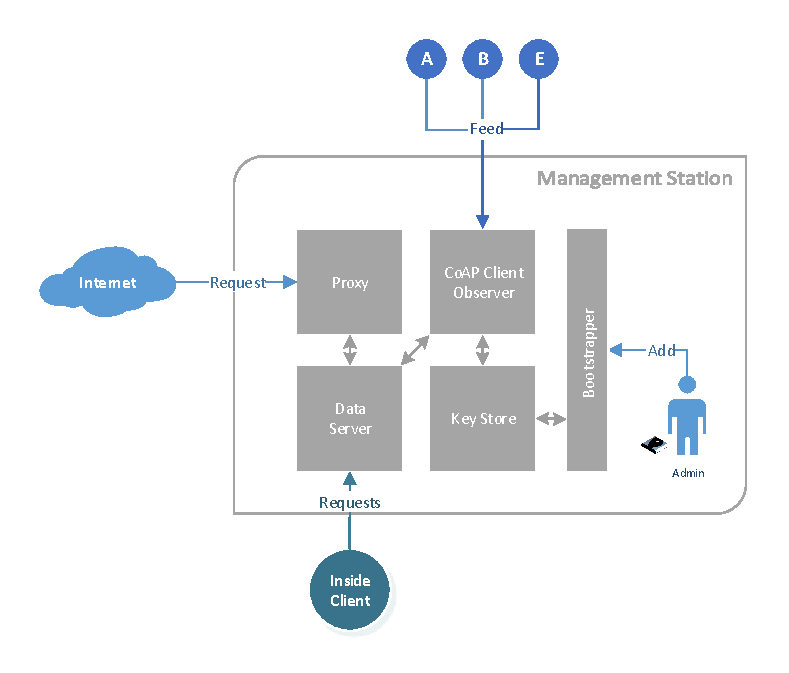
\includegraphics[width=0.92\linewidth]{figures/White_Box_Model.pdf}
  \caption{Central Management Station}
  \label{fig:core_components}
\end{figure}

\paragraph{\textbf{Credentials Configuration}}
\paragraph{}
In order to achieve secure communications, a new node must connect to the RPL network in a secure way, that is by using a pre-shared group key. After that network setup, it will also need to make a DTLS handshake with the client observer, for that needing a key pair and the public key of the client observer. That information is written into the device during the configuration phase, done by the staff members. Figure \ref{fig:sequence_bootstrapping} shows a sequence diagram of the initial configuration phase. This process will be fully automated without requiring the staff administrator any knowledge of the inner workings of the network and authentication procedures.

\begin{figure}[h]
  \centering
  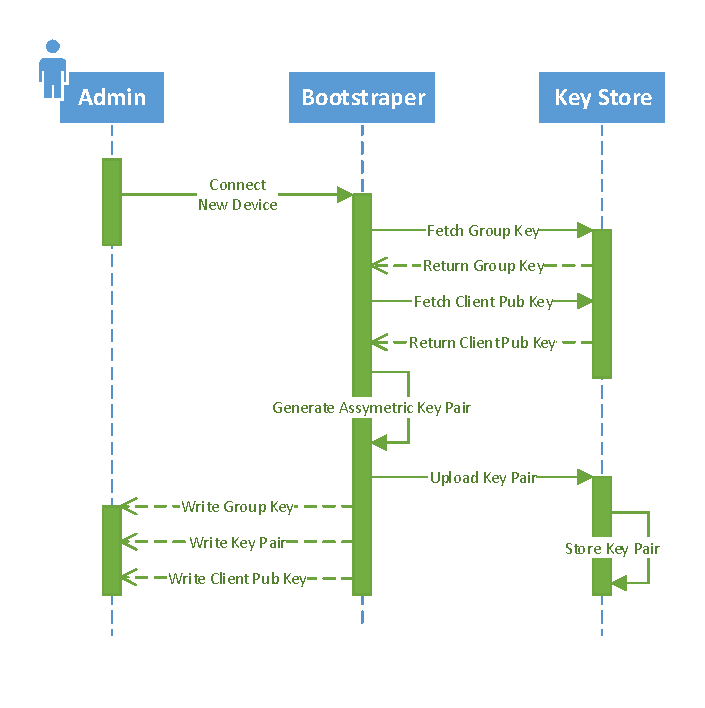
\includegraphics[width=0.8\linewidth]{figures/Sequence_Bootstrapping.pdf}
  \caption{New Device Initial Configuration}
  \label{fig:sequence_bootstrapping}
\end{figure}

As shown in the sequence diagram, the process is initiated by a staff member by connecting a new device to the bootstrapper. The bootstrapper automatically requests the network group key from the key store and the Client Observer public key. Then a new key pair is generated and stored in the key store for that device. Finally the bootstrapper writes the group key, the key pair and the Client Observer public key into the device.
\pagebreak
\paragraph{\textbf{Network Layer Bootstrapping}}
\paragraph{}

After the credentials configuration phase, the new device is fully equipped with the security credentials required for joining the RPL network. Figure \ref{fig:sequence_network_admission} shows a sequence diagram of the process started by the new node to join the network topology. The vocabulary used to represent the message exchange was previously presented in Section \ref{sec:network_layer}. All the message exchange is done with the secure versions of the RPL control messages, meaning the data is cyphered with the shared group key.

\begin{figure}[h]
  \centering
  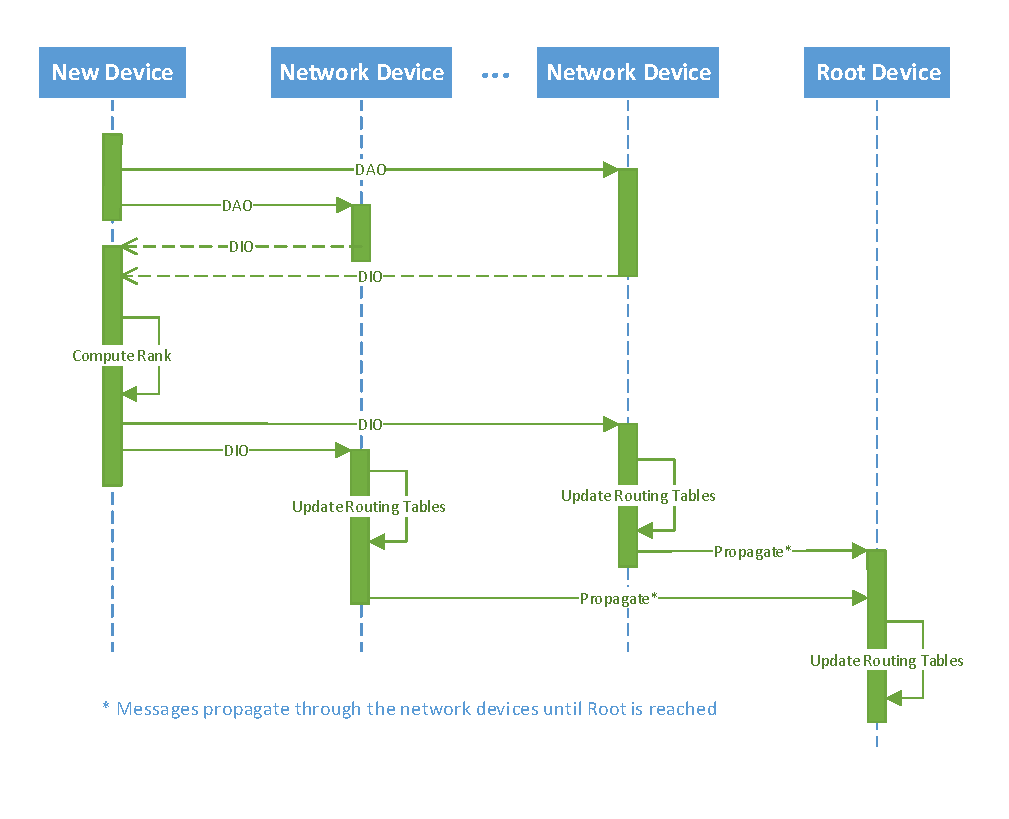
\includegraphics[width=1.0\linewidth]{figures/Sequence_Network_Admission.pdf}
  \caption{Network Layer Bootstrapping}
  \label{fig:sequence_network_admission}
\end{figure}

As shown in the sequence diagram, the process is initiated by the joining device by broadcasting \gls{DAO} messages to any available neighbour devices in range. The receiving nodes will reply to the new device with a \gls{DIO} message that provides graph routing information. With this information the new device is able to compute its rank (the distance towards the root) and define its parents based on that metric. After that process is complete, the new device tells his neighbours about its position in the graph using a \gls{DIO} message and the receiving nodes update their routing tables so that downwards traffic can now reach the new node. This information is further propagated up the network topology until the root is reached.

\vspace{20mm} %5mm vertical space

\paragraph{\textbf{Application Layer Bootstrapping}}
\paragraph{}

Although the device is now bootstrapped at the network layer, it still needs to discover and be discovered at the application layer. This means contacting the Client Observer, securing the channel through \gls{DTLS} and then send new readings as they occur. Figure \ref{fig:sequence_application_admission} shows a sequence diagram of the process started by the new node to join the \gls{CoAP} network.

\begin{figure}[h]
  \centering
  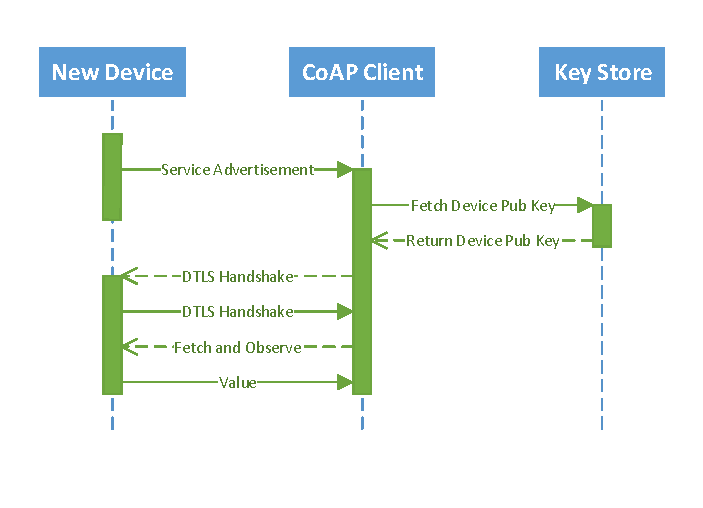
\includegraphics[width=0.8\linewidth]{figures/Sequence_Application_Admission.pdf}
  \caption{Application Layer Bootstrapping}
  \label{fig:sequence_application_admission}
\end{figure}

As shown in the sequence diagram the process is started by the new device that advertises its services to the network. That message is eventually received by the Client Observer who uses the new device public key, stored in the key store to start a \gls{DTLS} secured channel. After the handshake is completed, the Client Observer requests the latest readings to the sensor and sets the observe option meaning each time there is a change in the sensor reading the client will be notified.

\section{Implementation}

\subsection{Network Devices}

\paragraph{\textbf{Operative System}}
\paragraph{}
The greatest planning challenge involved in deploying the network devices was connecting all the proposed protocol at the different layers together. To achieve this, several operative systems for constrained devices were examined attempting to understand how they worked and what features did they offer. The operative systems under comparison were Contiki-OS\footnote{http://www.contiki-os.org/}, TinyOS\footnote{http://tinyos.stanford.edu/tinyos-wiki/index.php/FAQ} and RIOT-OS\footnote{https://riot-os.org/}\\
After examination of the source code repositories, wiki pages and community mailing lists, we could understand that RIOT is the newest and more ambitious, attempting real time processing and claiming to support "all relevant open standards" for the \gls{IoT} but still in a starting phase and lacking complete implementations of some protocols and still working on developing drivers for the most recent hardware platforms. Regarding TinyOS, it follows a less ambitious approach, presenting itself as a work scheduler with a collection of drivers for micro-controllers. Unfortunately, it appears to have stopped in time, with the latest release being dated August 2012 and not supporting the latest hardware boards. Contiki-OS on the other hand claims to be a "powerful box for building complex wireless systems". According to the documentation it supports all the protocols required and has recently published drivers for the most recent hardware platforms. It also ships with a network simulator, allegedly allowing to construct a virtual network that accurately mimics a real deployment on hardware. The combination of these factors led to the choosing of Contiki-OS as the operative systems for our network nodes. Figure \ref{fig:stack_operative_system} acts as a reminder of the attempted protocol stack, alongside with the selected operative system.\\

\begin{figure}[h]
  \centering
  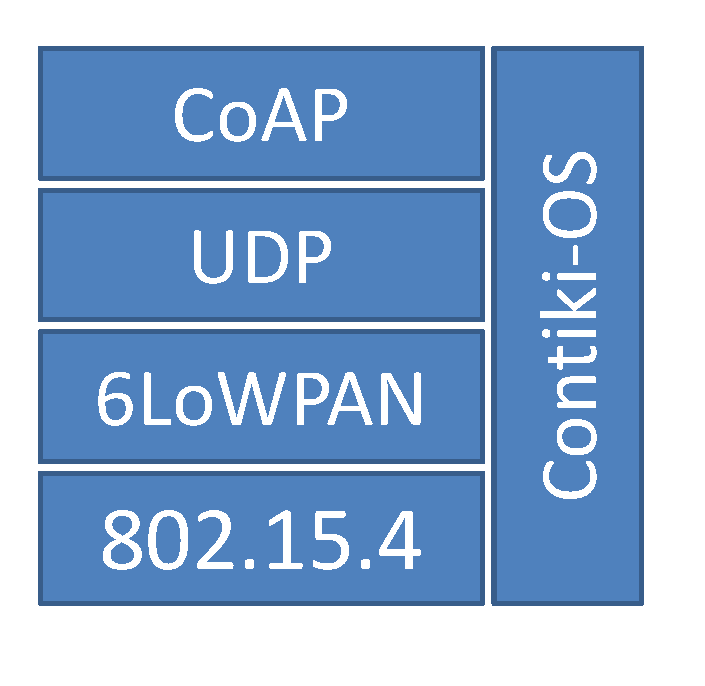
\includegraphics[width=0.3\linewidth]{figures/Stack.pdf}
  \caption{Protocol Stack and Operative System}
  \label{fig:stack_operative_system}
\end{figure}

With respect to the Contiki-OS internal structure, the operative system has been divided by category folders at the root level, similar to what can be found on a regular Linux distribution. The most relevant and that required greatest attention and understanding for this work are presented as follows:

\begin{itemize}
	\item \textbf{apps} - in this folder lies the code for applications, like telnet, ping, mqtt and our desired application layer protocol - \gls{CoAP};
	\item \textbf{core/net} - in this folder, the code responsible for networking is found, particularly our desired network layer protocol - RPL. IPv6 and link layer security are also implemented;
	\item \textbf{platform} - in this folder we can find the drivers for the supported platforms;
	\item \textbf{examples} - in this folder, simple working examples of many apps can be found, including \gls{CoAP};
	\item \textbf{tools} - in this folder we find non-essential apps that can help if we want for example to measure resource consumptions on real hardware.
\end{itemize}

\paragraph{\textbf{Application and Session Layer}}
\paragraph{}

Although applications should now come out-of-the-box with the selected operative system, \gls{CoAP} configuration and the creation of the application endpoints that will be accessed by the network clients on the management station needs to be done by the developer. These endpoints also increase in complexity when accessing specific hardware like humidity and temperature sensors, or when we want observable resources, where when a change occurs an event is triggered that will notify all the resource observers. In our work, we wanted to imprint on the devices an unique identifier, therefore needing to implement a simple text resource, and also make use of the hardware capabilities to create a live network, resorting to the sensors included on hardware. This implied the creation of endpoints capable of interacting with hardware devices and configuring those endpoints to be observable by the \gls{CoAP} clients. The following snippets present an overview of what is required for creating observable \gls{CoAP} endpoints.\\
Firstly, it is necessary to declare a new resource. Since we will be creating a temperature resource, and temperatures change without human intervention, it needs to be declared as n periodic resource in order to trigger periodic temperature reading events. Besides the title, it needs a handler function that runs when the endpoint is reached by a client, and a periodic handler function that runs when a specified amount of time is reached.

\begin{lstlisting}[caption={CoAP Periodic Resource Declaration}]
PERIODIC_RESOURCE(res_temperature,
         "title=\"Temperature\";rt=\"Temperature\";obs",
         res_get_handler,
         NULL,
         NULL,
         NULL,
         CLOCK_SECOND,
         res_periodic_handler);
\end{lstlisting}

The handler function is responsible for returning the most up-to-date value on the resource being requested. To do this, if first reads the latest value directly from hardware, and then construct the appropriate response using the fetched value.

\begin{lstlisting}[caption={CoAP Periodic Resource Handler}]
static void
res_get_handler(void *request, void *response, uint8_t *buffer, uint16_t preferred_size, int32_t *offset)
{

  int temperature = temperature_sensor.value(0);

  REST.set_header_content_type(response, REST.type.TEXT_PLAIN);
  snprintf((char *)buffer, REST_MAX_CHUNK_SIZE, "%d", temperature);

  REST.set_response_payload(response, (uint8_t *)buffer, strlen((char *)buffer));
  REST.set_header_max_age(response, MAX_AGE);
\end{lstlisting}

The periodic handler function is responsible for monitoring the resource and if it detects changes to the value, within a configured range, it sends messages to all the registered resource observers with the most up-to-date value.

\begin{lstlisting}[caption={CoAP Periodic Resource Periodic Handler}]
static void
res_periodic_handler()
{
  int temperature = cc2538_temp_sensor.value(1);

  ++interval_counter;

  if((abs(temperature - temperature_old) >= CHANGE && interval_counter >= INTERVAL_MIN) || 
     interval_counter >= INTERVAL_MAX) {
     interval_counter = 0;
     temperature_old = temperature;
    /* Notify the registered observers which will trigger the res_get_handler to create the response. */
    REST.notify_subscribers(&res_temp);
  }
}
\end{lstlisting}

Finally, the created resources need to be activated in the \gls{CoAP} main process so that they will become visible to clients requesting the resources that server is making available. Additionally, it is necessary to activate hardware specific components that are being used in those endpoints, in this case the temperature sensor. After these declarations are run, Contiki-OS will provide the necessary data structures and pointers to interact with the resource and make them available for the previously seen handlers. This is one of the big advantages of working with a operative system that supports both the application layer protocols and target hardware.

\begin{lstlisting}[caption={CoAP Resources Activation}]
PROCESS_THREAD(coap_server, ev, data)
{
  PROCESS_BEGIN();

  PROCESS_PAUSE();

  /* Initialize the REST engine. */
  rest_init_engine();

  /* Initialize project specific endpoints */
  rest_activate_resource(&res_id, "info/id");
  rest_activate_resource(&res_event, "sensors/button");
  rest_activate_resource(&res_temp, "sensors/temperature");

  /* Initialize board specific drivers */
  SENSORS_ACTIVATE(cc2538_temp_sensor);
  PROCESS_END();
}
\end{lstlisting}

After having a working \gls{CoAP} server, the focus moved to securing the communications at the session layer, as planned, using \gls{DTLS}. Unfortunately this goal was never achieved due to the lack of compatibility between the available \gls{DTLS} implementations, the used operative system and the selected hardware board. Although many attempts have been made, using implementations from different sources \footnote{https://github.com/cetic/6lbr/wiki/Example-:-Dtls-Coap-Server} a running setup was never achieved. As an extreme option, moving towards another operative system (TinyOS) was attempted, and even using the "supported" \gls{DTLS} implementation from that system, it was not possible to achieve a running example since it had only been tested on old hardware and was not working with the most up-to-date boards available. After submiting bug reports and trying to get help from the community with no practical results the usage of \gls{DTLS} was abandoned since the time required to adapt an existing implementation to our working setup would take more time than the available to complete this project.

\paragraph{\textbf{Network Layer}}
\paragraph{}

Regarding the implementations at the network layer, the desired routing protocol, \gls{RPL}, should work out-of-the-box with the selected operative system and indeed it did. However some small adjustments and configurations needed to be made so that the total amount of allocated space for routing tables could fit the target hardware. These tweaks were made in the \gls{RPL} configurations file and resorted to limiting the amount of neighbours and max-routes per device. A maximum of twenty routes and twenty neighbours was chosen since it was far superior to the required for this project and believed to be a reasonable number for the smart campus scenario under consideration.

\begin{lstlisting}[caption={RPL Configurations}]

#ifndef NBR_TABLE_CONF_MAX_NEIGHBORS
#define NBR_TABLE_CONF_MAX_NEIGHBORS                20
#endif
#ifndef UIP_CONF_MAX_ROUTES
#define UIP_CONF_MAX_ROUTES                 20
#endif

\end{lstlisting}

Once the network layer was working and it was possible to see the topology being formed, the focus moved to enable the secure variation of the \gls{RPL} messages that would authenticate them and prevent the vampires from joining the network. Unfortunately, when the developers of Contiki-OS implemented the \gls{RPL} protocol for their operative system, left out the secure variations of the protocol control messages as fixed in the \gls{RPL} RFC document \footnote{https://tools.ietf.org/html/rfc6550}. Since this was a mandatory feature for the whole purpose of this work, alternatives needed to be found, and after contacting the developers behind the \gls{RPL} implementation for Contiki-OS, we were advised to use \gls{LLSec} as an alternative.\\
\gls{LLSec} works by cyphering packets at the link-layer, right before leaving the host. Those packets are then deciphered upon reaching the next device. This process repeats itself until the destination is reached. In the case of Ad-Hoc networks like this one, the proposed alternative was achievable, and an implementation of \gls{LLSec} was already present in Contiki-OS. To make use of \gls{LLSec}, a network-wide key needed to be flashed onto the hardware that would then be used for the packet cyphering. More in depth, the security credential provided to the joining nodes is a 128bit key, used for the \gls{AES} \cite{Fips2001} in \gls{CCM} star mode \cite{Corp2005}. This allows packets to have their payload encrypted and the message authenticated with a \gls{MIC} also computed from the AES-128 key. This assures that all the packets flowing through the network, even the joining node first communications, are confidential and authentic therefore fulfilling the requirements for this layer. Further explanations of this bootstrapping phase will be given in the Central Management Station section \ref{backend_services}.

\subsection{Border Router}

The border router is the network component that creates the bridge between the \gls{6LoWPAN} network and the outside world. This means that the device will need to have two interfaces, one with the 802.15.4 radio and another one to connect to the outside networks. The border router can and should be permanently connected to a power source, meaning that its power consumption is not an issue. Also, it should be more powerful than the remaining network devices because it will be in charge of taking care of all the packets going inside and outside the \gls{6LoWPAN} network. After analysing the available border router solutions, the implementation from \gls{CETIC} \footnote{https://github.com/cetic/6lbr/} was selected because it provides a deployment-ready solution that runs out-of-the-box on Linux hosts, supports various network topologies, is in active development, has releases from this year (2016) and an active community. Considering this option, the well known Raspberry Pi \footnote{https://www.raspberrypi.org/} board was selected to be the host of the \gls{CETIC} solution due to its more capable hardware, widespread use and full support from the border router distribution. Since the Raspberry platform does not possess an 802.15.4 radio interface, one of the network hardware boards was used as the radio for the border router, a solution that is also fully supported by the \gls{CETIC} distribution. Figure \ref{fig:border_router_setup} shows the border router setup used for this work and its connections to the central management station

\begin{figure}[h]
  \centering
  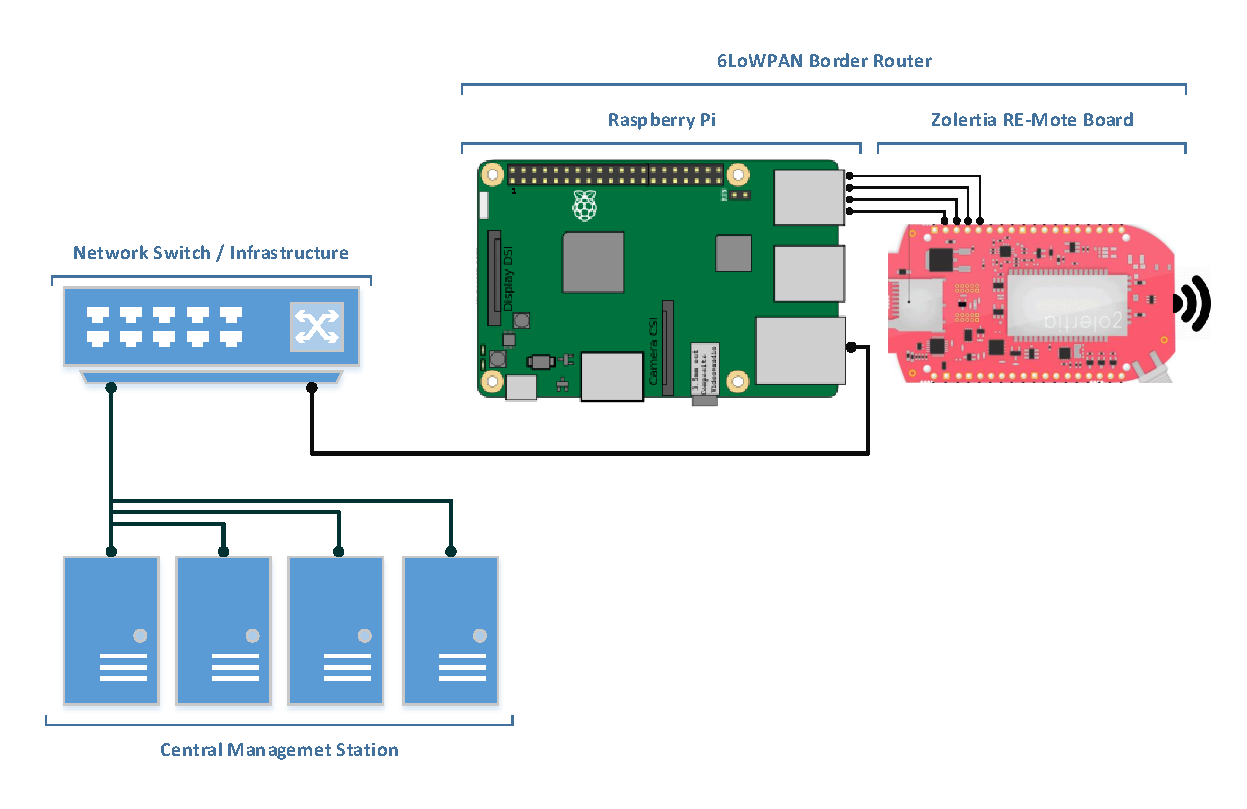
\includegraphics[width=1.0\linewidth]{figures/Border_Router.pdf}
  \caption{Border Router Setup}
  \label{fig:border_router_setup}
\end{figure}

For the border router to become active, firstly a Linux distribution needs to be installed on the device. In this work, the Raspbian \footnote{https://www.raspberrypi.org/downloads/raspbian/} distro was used due to its widespread use and support. Then, \gls{CETIC}'s border router implementation needs to be installed as a service running on the Linux host. This is done by firstly installing the required dependencies, followed by compiling the sources and then starting the service.

\begin{lstlisting}[caption={Border Router Dependencies and Installation}]

sudo apt-get install libncurses5-dev
sudo apt-get install bridge-utils

make all
make plugins
make tools

sudo make install
sudo systemctl daemon-reload
sudo service 6lbr start

\end{lstlisting}

Now all that is left to do is flash the hardware board providing 802.15.4 communications. Within the sources for the border router we can find the executables for flashing this board with the slip radio firmware. This can be done with the following command:

\begin{lstlisting}[caption={Firmware Upload Command}]

make TARGET=remote slip-radio.upload

\end{lstlisting}

In the case of plain-text communications, no additional steps were required for operation, and the border router solution should be working as the topology root and immediately adding any servers within reach to the network. However, since our solutions makes use of \gls{LLSec} it is required that the border router learns the network key. The border router will always be the destination of all packets going outside the \gls{6LoWPAN} network and the final deciphering point for the message packets. This can be done on the border router administration page as presented in Figure \ref{fig:administration_page}.

\begin{figure}[h]
  \centering
  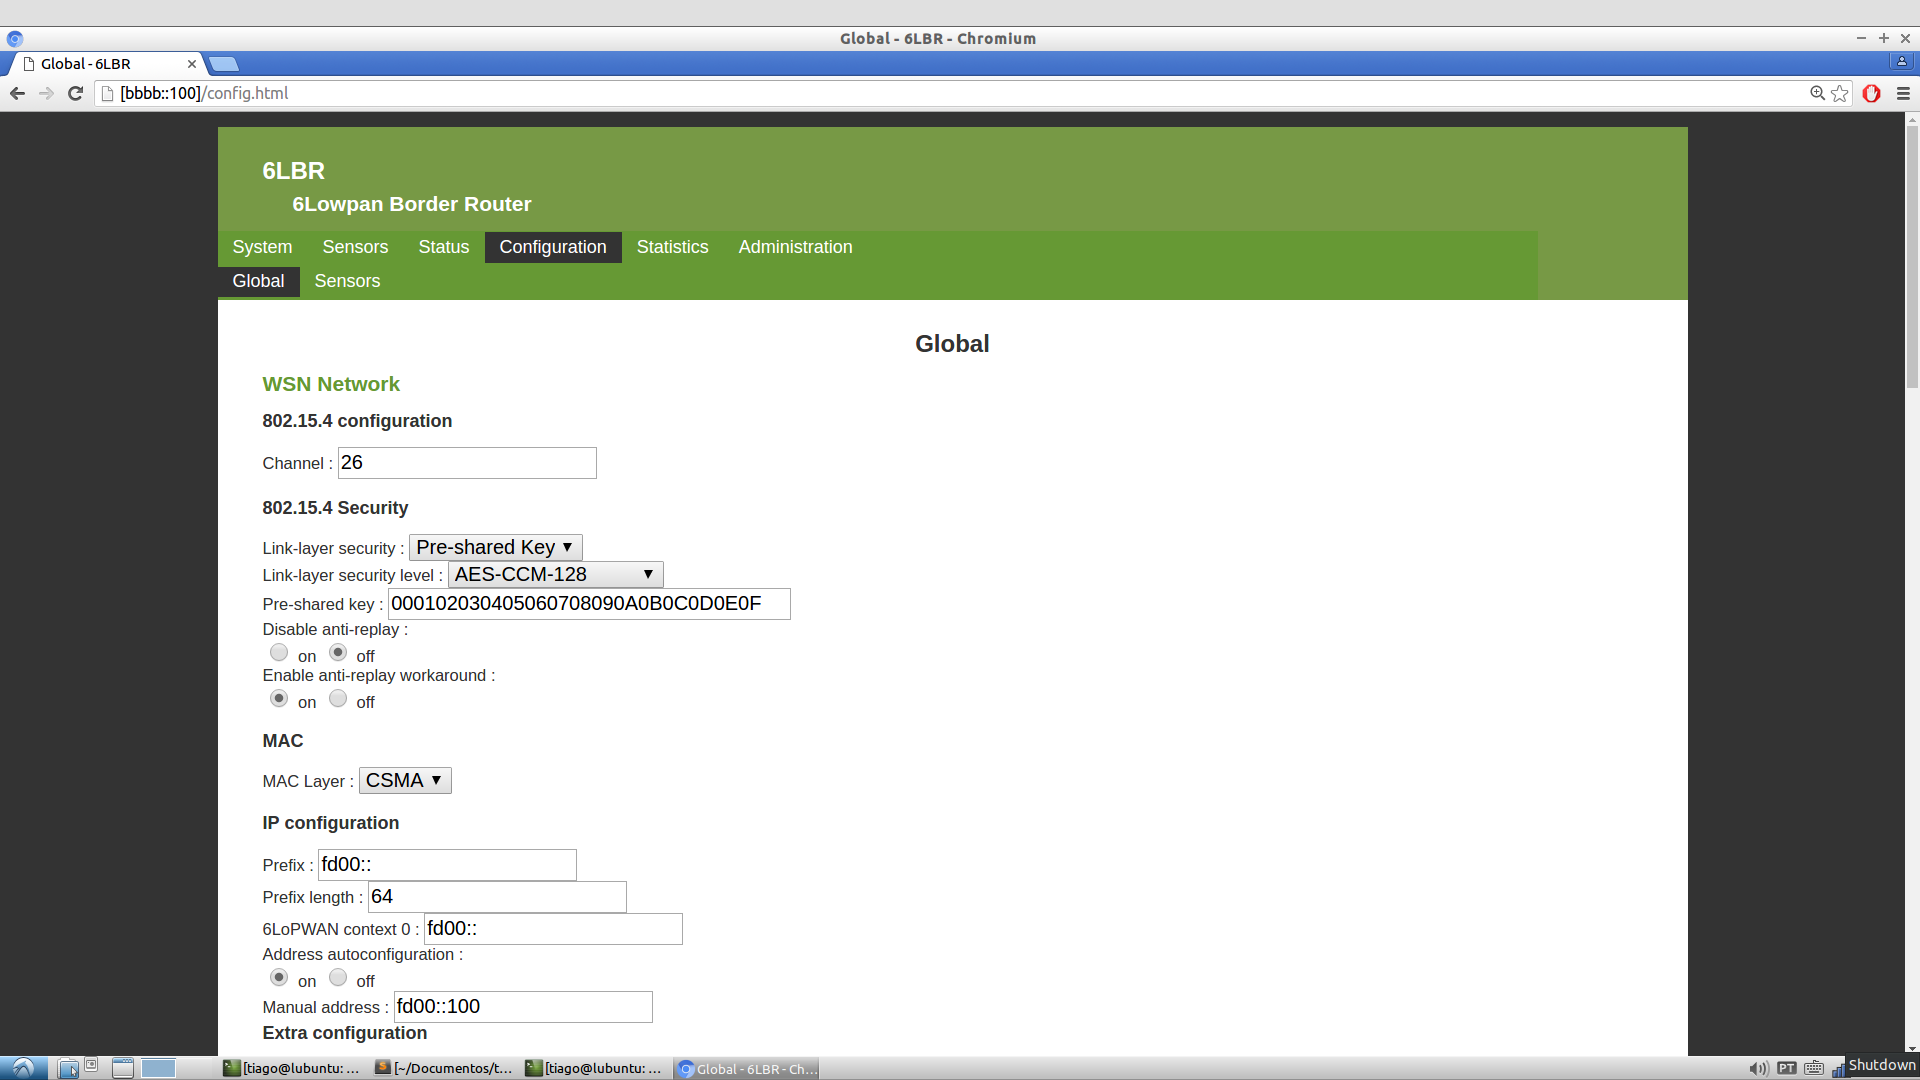
\includegraphics[width=0.95\linewidth]{figures/border_router_page.png}
  \caption{Border Router Administration Page}
  \label{fig:administration_page}
\end{figure}

\subsection{Central Management Station}
\label{backend_services}

The central management station is in charge of fetching the most up-to-date values of the network devices, storing them and allowing access to outside client. Although without the usage of \gls{DTLS} some of the station components are now more simple, there is still an important collection of previously presented pieces that come into play. The following paragraphs show how they were implemented and their role in the station. For simplicity and easier setup, all the pieces of the management station were deployed on a single machine, however in real application they could be divided into separate physical machines for improved performance.

\paragraph{\textbf{Data Server and Key Store}}
\paragraph{}
The role of the Data Server is to store the latest values received by the \gls{CoAP} Client and provide them on demand to the outside network clients. It was implemented resorting to two pieces, a database and a webserver. The selected webserver is the well known Apache \footnote{https://httpd.apache.org/} due to the extensive amount of documentation and previous experience with this server. It is important to state that other from installing the service from the Linux distribution repositories, a certificate should be used to ensure the safety of communications between the network clients and the central management station. For the purposes of this work, and since all is to be demonstrated locally, this certificate was not requested or put in production. The webpage being served by the Apache server is used for the bootstrapping process and to monitor the network status and latest values. Screenshots of this webpage are provided on the System Execution section \ref{sec:system_execution}.\\
Regarding the database, a Mysql \footnote{https://www.mysql.com/} instance was used, once again due to the extensive amount of documentation and previous experience. Since there is not the need to store public/private keys, the network-wide key used for the \gls{LLSec} was directly stored and accessed on this same database. The database holds the following information:

\begin{itemize}
  \item \textbf{Authorized Nodes} - the nodes that are authorized to belong to the network. Holds information about there unique identifier, name, type, zone and IP address;
  \item \textbf{Network Keys} - the keys used for the \gls{LLSec}. Holds information about the current key. Is updated in the administration console and is fetched when a new node goes through the bootstrapping process;
  \item \textbf{Node Resources} - the resources each network nodes has endpoints to. Holds information about their type, endpoint and latest value. Is updated by the \gls{CoAP} client and is fetched by the network clients;
  \item \textbf{Supported Hardware} - the boards that are supported by the bootstrapper. Holds informations about their name and type and is used during the bootstrapping phase to flash new devices appropriately.
\end{itemize}


\paragraph{\textbf{CoAP Client Observer}}
\paragraph{}

The client observer plays a very important role in the network because is in charge of discovering the \gls{CoAP} servers, contacting them and fetching the most up-to-date values from them. This process was implemented in three steps. Firstly, the process needs to discover the active servers on the network. It does this by parsing the border router administration page looking for the devices in the topology and their address on the \gls{6LoWPAN} network. To facilitate the web crawling part JSoup \footnote{https://jsoup.org/} was used. After learning about the active servers, the process creates \gls{CoAP} client objects so that their endpoints can be reached. The client objects belong to the Californium Framework \footnote{http://www.eclipse.org/californium/} being used on the Java project.  

\begin{lstlisting}[caption={CoAP Client Device Discovery}]

public static List<String> parse (String url) throws IOException{
		
		List<String> nodes = new ArrayList<String>();
		
		Document doc = Jsoup.connect(url).get();
		Elements rows = doc.select("tr");
		for (Element row : rows) {
		   Element node = row.select("td").get(0);
		   String nodeText = node.text();
		   
		   //don't insert table header
		   if(!nodeText.equals("Node")){
			   nodes.add(nodeText);
		   }
		}
		
		return nodes;
}

private void processBorderRouter() throws IOException, NumberFormatException, SQLException{

		List<String> ips = BorderRouterCrawler.parse("http://[bbbb::100]/sensors.html");
		
		for(String ip : ips){
			CoapClient idFetcher = new CoapClient(PROTOCOL, "["+ip+"]", PORT, "info", "id");
			CoapResponse response = idFetcher.get();
			String keyCode = response.getResponseText();
			dbutils.setIP(Long.parseLong(keyCode), ip);
		}
		
		System.out.println("[BR-PARSER] - Parsing Completed");
}

\end{lstlisting}

Secondly, the process needs to request the discovered servers their available resources and register the created \gls{CoAP} clients on their endpoints. Thirdly, a handler functions needs to be created so that when new values are received the database gets updated. In the following snippet, the handler code for a temperature update is shown. 

\begin{lstlisting}[caption={CoAP Client Resource Handling}]

CoapClient tempObserver = new CoapClient(PROTOCOL, "["+node.getIp()+"]", PORT, "sensors", "temperature");
				CoapObserveRelation tempRelation = tempObserver.observe(
					new CoapHandler() {
						@Override public void onLoad(CoapResponse response) {
							String content = response.getResponseText();
							String[] output = response.advanced().getSource().getHostAddress().split(":");
							StringBuilder ipBuilder = new StringBuilder();
							for(int i = 0; i < output.length; i++){
								if(!output[i].equals("0")){
									ipBuilder.append(output[i]);
									if(i == 0){
										ipBuilder.append(":");
									}
									if(i != output.length-1){
										ipBuilder.append(":");
									}
								}
							}
							String ip = ipBuilder.toString();
							System.out.println("[NEW-TEMP] IP: " + ip + " | TEMP(mC):" + content);
							try {
								dbutils.setTemperature(ip,content);
							} catch (SQLException e) {
								System.out.println("error updating temperature on DB:");
								e.printStackTrace();
							}
						}
						
						@Override public void onError() {
							System.err.println("OBSERVING TEMP FAILED (press enter to exit)");
						}
					});


\end{lstlisting}

This process keeps running in the background fetching new servers and updating database values based on the received updated on the handler functions.

\paragraph{\textbf{Bootstraper}}
\paragraph{}

The bootstraper is the central management station that directly interfaces with the hardware boards and attempts to facilitate the installation of new devices. It provides a USB interface for the new device to be physically connected during the flashing and uses the web server pages for guiding the user during the firmware upload. After the device is connected, the bootstrapper will require the user to select the target hardware and a name for the device. Then it will create new entries in the database for the new device and proceed to compile a \gls{CoAP} server. Finally it will fetch the network key to be used on the \gls{LLSec} and flash it alongside with the Contiki-OS firmware. The script that runs in the background is the following:

\begin{lstlisting}[caption={Bootstrapper Credentials Flashing Script}]

$llsec = str_split(getKeys()[0], 2);
  $formated_llsec = "#define NONCORESEC_CONF_KEY {";
  $size = count($llsec);
  for($i = 0; $i < $size; ++$i){
	if($i!=0){
	   $formated_llsec.= ",0x".$llsec[$i];
	} else{
	   $formated_llsec.= "0x".$llsec[$i];
	}
   }
  $formated_llsec.="}";
  
  $llsec_file_path = $CONTIKI_BASE_DIR."/bootstrap-key.h";
  $file = fopen($llsec_file_path, 'w');
  fwrite($file, $formated_llsec);
  fclose($file);
  
  $keycode = '#define ID '.$_POST['id'];
  print_r($keycode);
  $keycode_file_path = $CONTIKI_BASE_DIR."/resources/bootstrap-id.h";
  $file = fopen($keycode_file_path, 'w');
  fwrite($file, $keycode);
  fclose($file);
  $cmd_clean = "sudo make clean -C ";
  $cmd_make = "sudo make -C ";
  
  $cmd_target = $CONTIKI_BASE_DIR." TARGET=";
  $cmd_upload = " er-example-server.upload";
  $device = escapeshellarg($_POST['device']);
  
  $cmd_full_clean = $cmd_clean.$cmd_target.$device;
  $cmd_full_flash = $cmd_make.$cmd_target.$device.$cmd_upload;
  
  exec("/home/tiago/workspace/parallax/scripts/flash.sh '$cmd_full_clean'");
  exec("/home/tiago/workspace/parallax/scripts/flash.sh '$cmd_full_flash'");
  
\end{lstlisting}

After the device is flashed with the custom firmware it is ready to be deployed on the field. In order to facilitate the understanding of the system, the following section will provide a full execution scheme from the bootstrapping process to the observation of new values on the web page.

\section{System Execution}
\label{sec:system_execution}

This execution assumes that: the border router is already installed and running, the slip radio is already installed and running, all the components in the central management station are running. However it also assumes that this is the first execution so the network key needs to be added to the database for the bootstrapper to use.\\

Firstly, the operator starts by connecting the new device onto the USB port of the bootstrapper.
Secondly, it does the initial configuration of letting the bootstrapper know what is the network key to be used in future hardware installations. This is done on the Setup tab as despicted in Figure \ref{fig:bootstraper-setup-page}.

\begin{figure}[h]
  \centering
  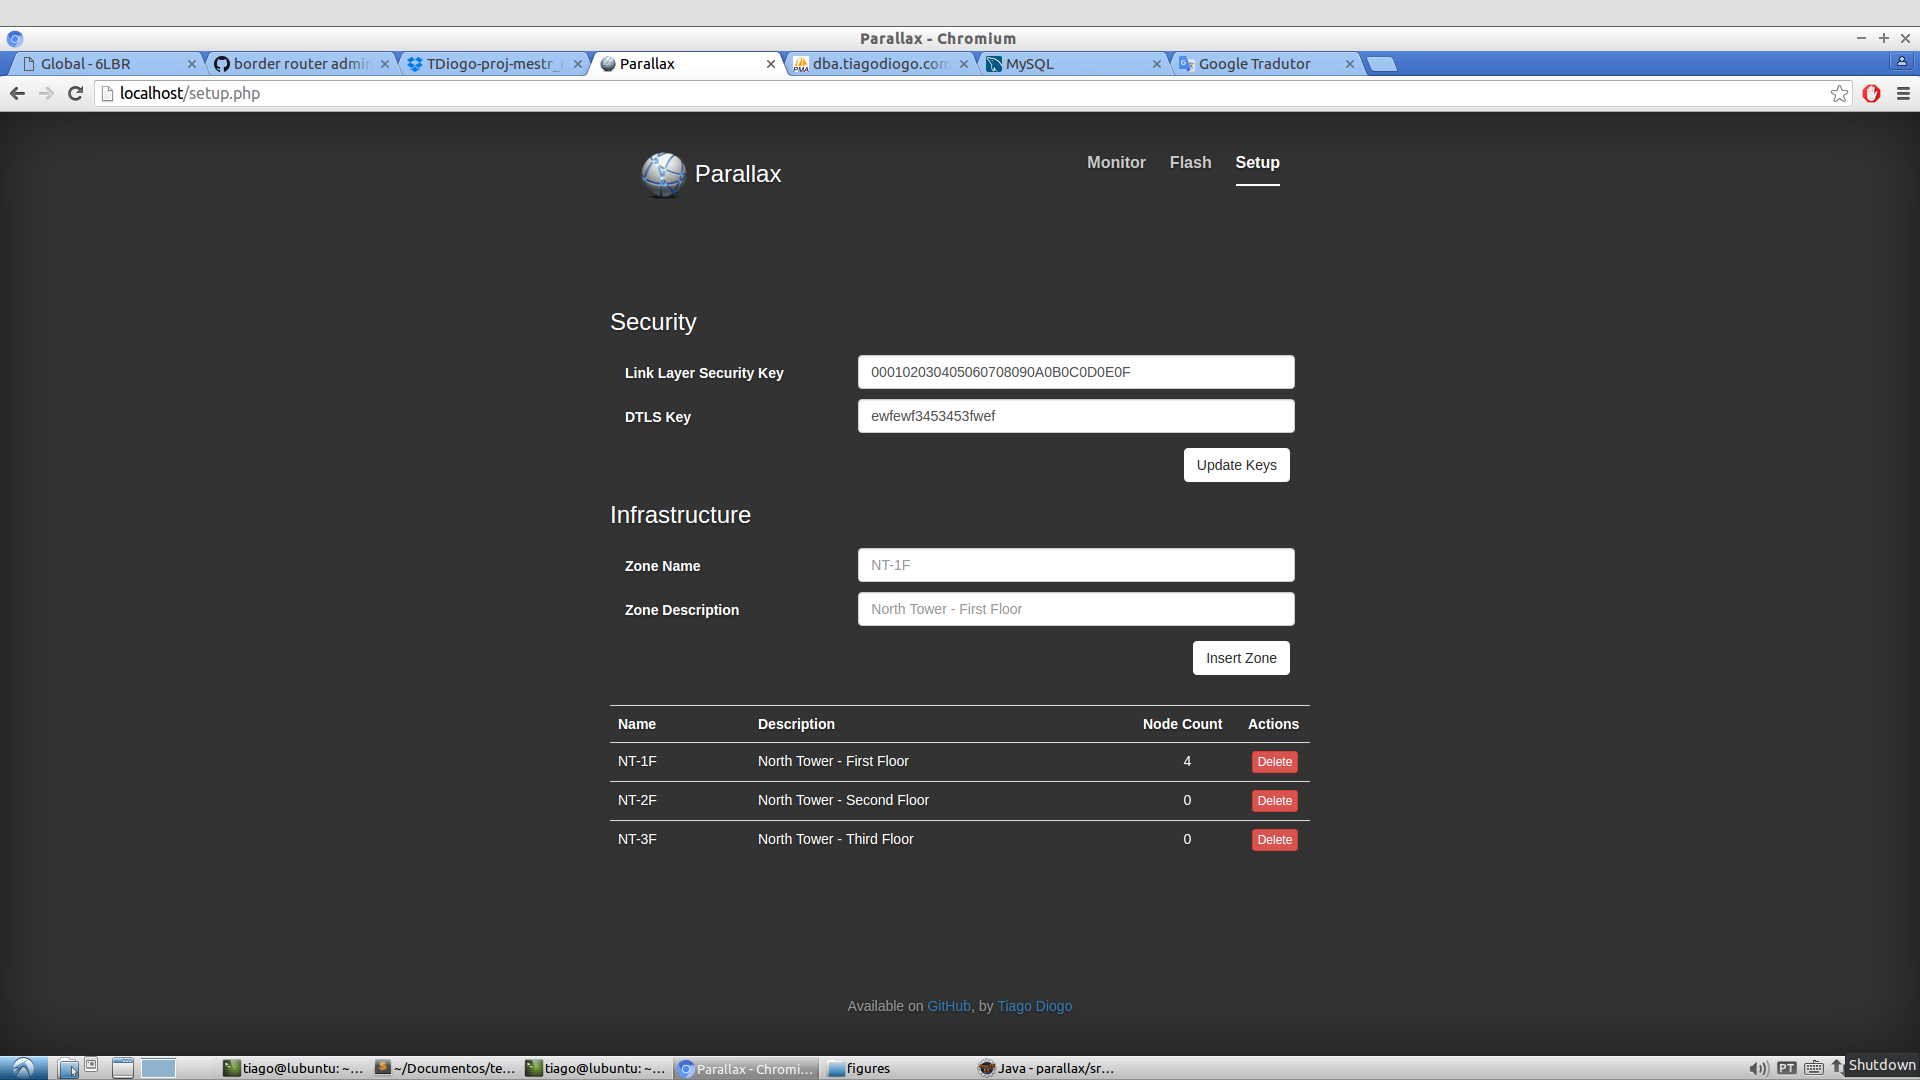
\includegraphics[width=0.7\linewidth]{figures/parallax_setup.png}
  \caption{Bootstraper Setup Page}
  \label{fig:bootstraper-setup-page}
\end{figure}

Here, the operator is also able to define infrastructure zones for better network organization. Each zone can be a building floor on our Smart Campus Scenario.\\
After doing this one-time setup, the operator can now proceed to the flashing stage, were the operative system alongside with the protocol stack and network key will be uploaded into the new device. To do this, all the operator needs to do is open the Flash tab, give a name to the new device, select the hardware type and the features he wishes to flash the device with. After this selection, with the touch of a button the new device will receive the customized firmware. The Flash tab is shown in Figure \ref{fig:bootstraper-flash-page}.

\begin{figure}[h]
  \centering
  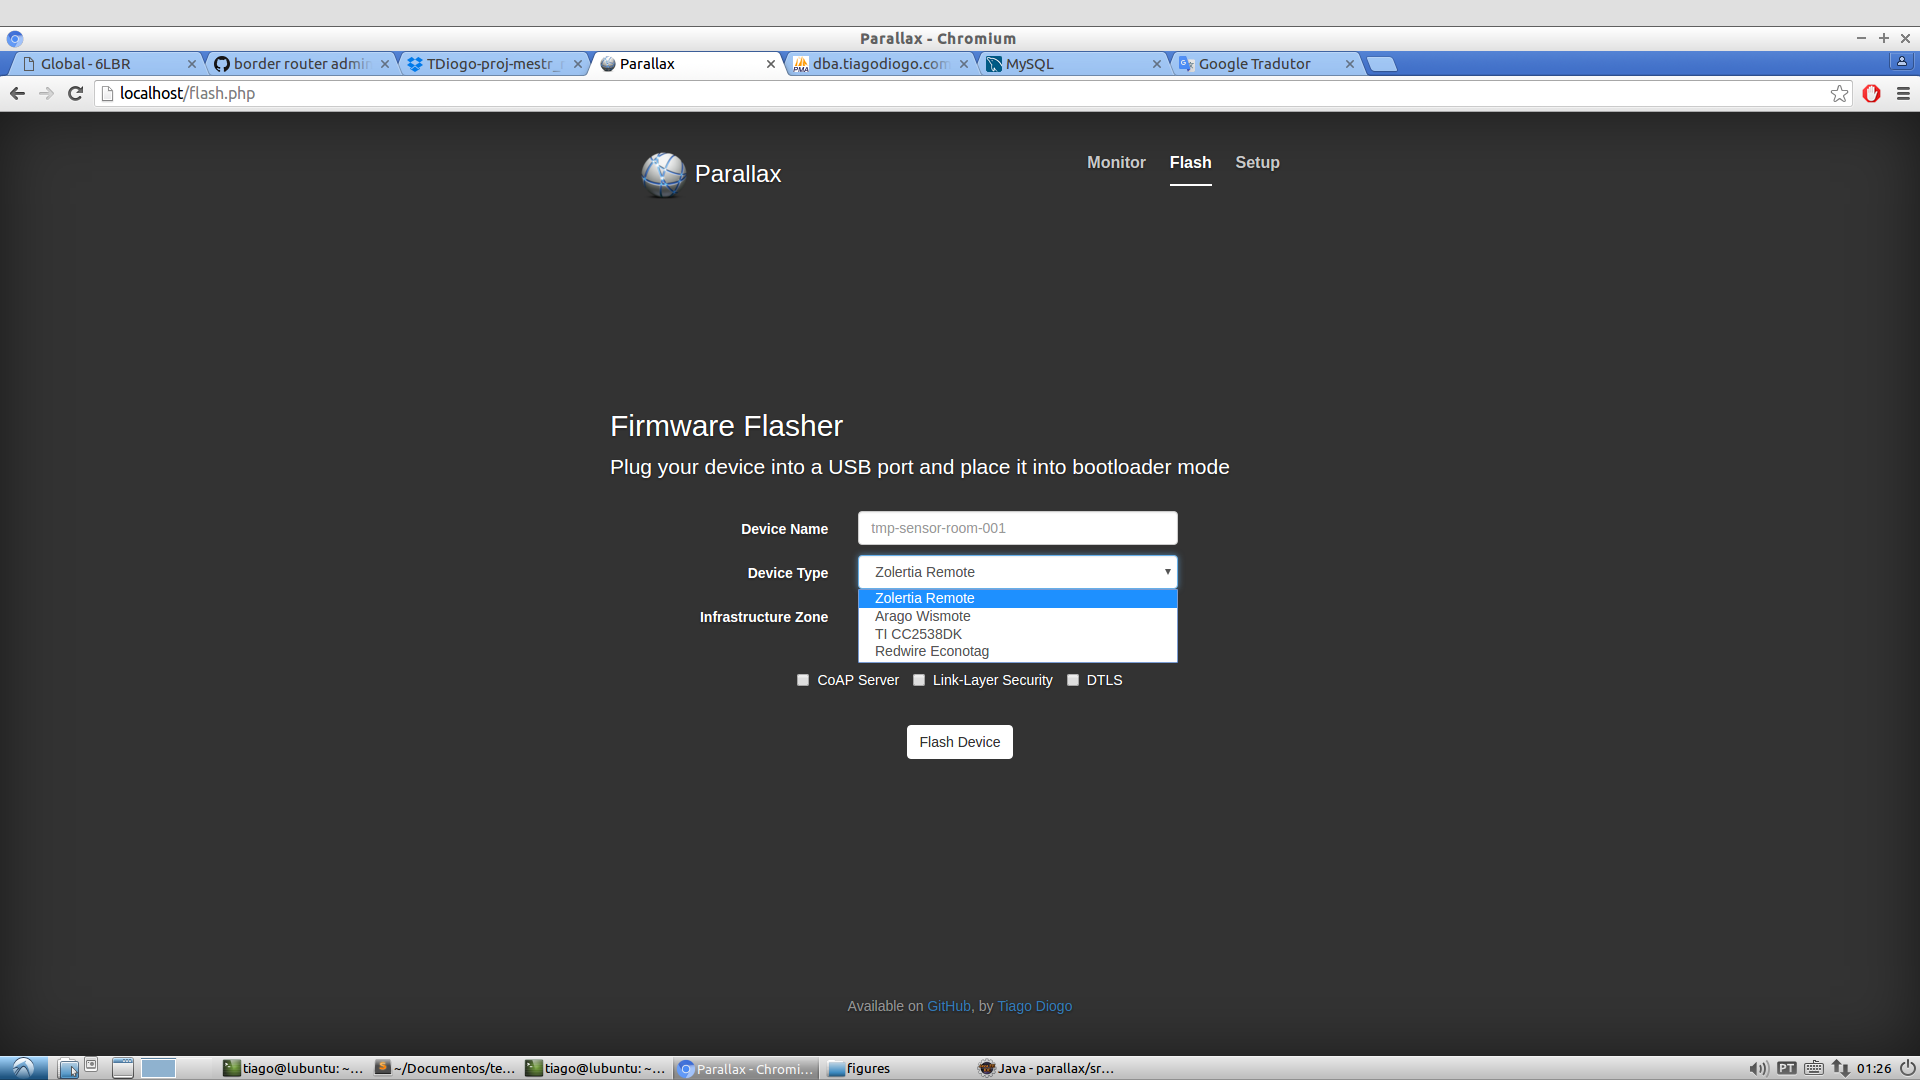
\includegraphics[width=0.7\linewidth]{figures/parallax_flash.png}
  \caption{Bootstraper Flash Page}
  \label{fig:bootstraper-flash-page}
\end{figure}

After this step, the new device is ready for commissioning on the field. Once it connects itself to the network, the observer on the central management station will notice an update on the topology of connected devices and try to register himself on the available server endpoints. Moments after, the most up-to-date reading from that server will be available for consulting on the Monitor tab, available for network clients and operators to use. The Monitor tab is shown in Figure \ref{fig:bootstraper-monitor-page}.

\begin{figure}[h]
  \centering
  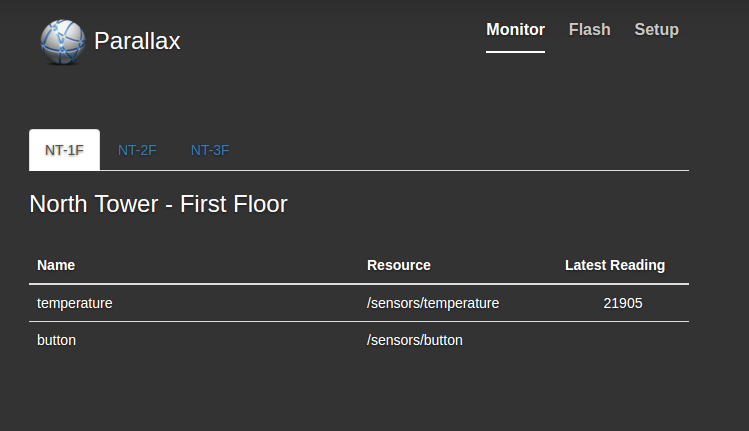
\includegraphics[width=0.8\linewidth]{figures/parallax_monitor.png}
  \caption{Bootstraper Monitor Page}
  \label{fig:bootstraper-monitor-page}
\end{figure}